\documentclass[a4paper]{jpconf}
 
\usepackage{float}
%\usepackage{amsmath} 
%\usepackage{amssymb}
%\usepackage{amsfonts}
\usepackage{epstopdf}
\usepackage{color,fancybox,graphicx}
\usepackage{url}
\usepackage{psfrag}
\usepackage{color}
\usepackage{pifont}
\usepackage{graphicx,rotating,booktabs}
\usepackage{xcolor}
\usepackage{iopams}
%\usepackage{amsthm}

\usepackage{amssymb,amsmath,amsthm,amsfonts}
\usepackage{framed}
\usepackage{mdframed}

\usepackage{enumitem}

\usepackage{lineno}
\linenumbers



\newtheoremstyle{my_theorem_style}
  {10pt} % Space above
  {10pt} % Space below
  {} % Body font
  {} % Indent amount
  {\bfseries} % Theorem head font
  {\\} % Punctuation after theorem head
  {.5em} % Space after theorem head
  {} % Theorem head spec (can be left empty, meaning `normal')

\theoremstyle{my_theorem_style}


\newtheorem{theorem}{Theorem}

\usepackage[ruled,vlined]{algorithm2e}

\usepackage[small,bf]{caption}
\setlength{\captionmargin}{25pt}

%\definecolor{}{rgb}{0.0, 0.5, 0.3}
%\definecolor{newblue}{rgb}{0.0, 0.1, 0.7}


\bibliographystyle{iopart-num}

%\usepackage{geometry}
%\geometry{a4paper, left=30mm, right=30mm, top=30mm, bottom=30mm, nohead}

\setlength{\parindent}{0cm}
\numberwithin{equation}{section}

\usepackage{tikz}

%\usepackage{hyperref}
%\hypersetup{
 % colorlinks = true,
 % urlcolor = blue, 
 % linkcolor = blue,
 % citecolor = newgreen,
%}
%\usepackage{subcaption}



\tikzstyle{state}=[shape=circle,draw=blue!50,fill=blue!20]
\tikzstyle{observation}=[shape=rectangle,draw=orange!50,fill=orange!20]
\tikzstyle{lightedge}=[-,dotted]
\tikzstyle{mainstate}=[state,thick]
\tikzstyle{mainedge}=[<-,thick]
\tikzstyle{line} = [draw,thick,-latex]
\usetikzlibrary{positioning}
\tikzstyle{transition} = [font=\small]
\usetikzlibrary{calc}

\newtheorem{rem}{Remark}[section]
\newtheorem{defi}{Definition}[section]
\newtheorem{lem}{Lemma}[section]
\newtheorem{cor}{Corollary}[section]
\newtheorem{pro}{Proposition}[section]
\newtheorem{theo}{Theorem}[section]
\newtheorem{fact}{Fact}[section]
\newtheorem{exm}{Example}[section]


\newcommand{\N}{\mathbb N}
\newcommand{\R}{\mathbb R}
\newcommand{\prob}{\mathbb{P}}
\newcommand{\esp}{\mathbb{E}}
\newcommand{\inde}{\perp\!\!\!\perp}
\newcommand{\ra}{\rightarrow}

\newcommand{\bP}{\boldsymbol P}
\newcommand{\bC}{\boldsymbol C}
\newcommand{\bfP}{\bf P}
\newcommand{\bfC}{\bf C}
\newcommand{\bsi}{\boldsymbol}
\newcommand{\bis}{\boldsymbol\nu}
\newcommand{\ps}{\psi_n (\delta)}
\DeclareMathOperator*{\argmin}{arg\,min}
\DeclareMathOperator*{\argmax}{arg\,max}
\newcommand{\red}{\color{red}}


%----------------------------------------------------------
\begin{document}


\title{Active Muon Shield for the SHiP Experiment at CERN}
\author{A.~Baranov$^{1,2,\star}$, E.~Burnaev$^{3}$,  D.~Derkach$^{1,\star}$, A.~Filatov$^{1,\star}$,
  N.~Klyuchnikov$^{3}$,  O. Lantwin$^{4,\star}$, F.~Ratnikov$^{1,2,\star}$,
  A.~Ustyuzhanin$^{1,2,\star}$  and
 A.~Zaitsev$^{3}$
}
\address{$^1$ National Research University Higher School of Economics,  Moscow, Russia \\
$^2$ Yandex School of Data Analysis, Moscow, Russia \\
$^3$ Skolkovo Institute of Science and Technology, Moscow, Russia \\
$^4$ Imperial College London, London, UK \\
$^\star$ on behalf of the SHiP Collaboration}
\ead{filatovartm@gmail.com}

\begin{abstract}
The SHiP experiment is designed to search for very weakly interacting particles beyond the Standard Model which are produced in a 400 GeV/c proton beam dump at the CERN SPS. An essential task for the experiment is to keep the Standard Model background level negligible. In the beam dump, around $10^{11}$ muons will be produced per second. The muon rate in the spectrometer has to be reduced by at least four orders of magnitude to avoid muon-induced backgrounds. It is proved that novel active muon shield may be used to magnetically deflect the muons out of the acceptance of the spectrometer.
\end{abstract}

\date{\today}



\section{Introduction}
\label{intro}
The Standard Model of elementary particles despite its enormous success has several places for improvement~\cite{Ellis:2009tp}. In particular, the baryon asymmetry of the Universe~\cite{Asaka:2005pn} and a Dark Matter existence are yet to be explained. Heavy Neutral Leptons (HNLs)~\cite{Asaka:2005an}, which are right-handed partners of the Standard Model neutrinos should they be discovered will give a boost in our understanding of both above mentioned riddles of Nature. The existence of such particles is strongly motivated by theory and were searched extensively previously. Cosmological constraints on the properties of HNLs now indicate that the majority of the interesting parameter space for such particles was beyond the reach of the previous searches at the PS191~\cite{Bernardi:1985ny}, BEBC~\cite{CooperSarkar:1985nh}, CHARM~\cite{Bergsma:1985is}, CCFR and NuTeV~\cite{Vaitaitis:1999wq} experiments. 

For this reasons, a new fixed-target experiment at the CERN SPS accelerator was proposed~\cite{Bonivento:2013jag}. This experiment will use a 400~GeV proton beam on a fixed target to produce a large number of charm mesons. The HNLs from charm meson decays have a significant polar angle with respect to the beam direction, approximately 50 mrad on average. In order to maximise the geometric
acceptance for a given transverse size of the detector, the detection volume must therefore be placed
as close as possible to the target. The production of the charm mesons is accompanied by copious direct production of pions, kaons and short-lived light resonances. The subsequent decays of these particles would result in a large flux of muons and neutrinos. To minimise these decays, a combination of a target and a hadron absorber of a few metres length, both made of as dense a material as possible, is required. To reduce the detector occupancy and backgrounds induced by the residual muon flux, a muon shield is required downstream of the hadron absorber. The experimental set-up must therefore balance the opposing requirements of locating the detector as close as possible to the target and of accommodating a sufficiently long muon shield upstream of the fiducial volume of the detector to reduce muon-induced backgrounds.

\section{Bayesian Optimization}
The main goal of our research was to find a light and efficient
magnetic shield. In order to achieve this, we applied a Bayesian optimization algorithm. In this section we give an introduction to this method and motivation behind this approach.

Let $f(x)$ be a black-box function on $X \subset R^d$, which does not have an analytic expression and can be evaluated at a specific point only by conducting computationally intensive simulations, which in turn can yield noisy observations of the form $y_i = f(x_i) + \epsilon_i$, where $\epsilon_i$ is the random variable with zero mean and constant variance. Our ultimate goal is to find a point $x_*$ where $f(x_*)$ is a true global optimum (henceforth without loss of generality we will consider a maximisation problem). In this problem setup, the general framework for optimum searching iteratively constructs the sample $D_N = \{(x_i, y_i)\}_{i=1…}^N$, each iteration consists of three steps:
\begin{enumerate}
\item \label{point_choosing} Choose a new point $x_{i}$ for simulation 
\item Conduct simulations to obtain $y_{i} = f(x_{i}) + \epsilon_i$
\item If a stopping criterion is not met, add $(x_{i}, y_{i})$ to the sample $D_N$ and proceed to iteration $i+1$
\end{enumerate}
Convergence to the exact solution of the problem may require infinite amount of iterations, however, under some theoretical assumptions any degree of its approximation can be obtained within the corresponding finite horizon.

\begin{theorem}
If $f(x)$ is Lipschitz-continuous with a Lipschitz continuity constant C, $X$ is a $d$-dimensional unit hypercube, then in the noise-free case for any $\varepsilon  > 0$ some point $x_+$ with near-optimal true value $f(x_+)$ : $f(x_+) \geq \max_{x \in X}f(x) - \varepsilon $ is guaranteed to be found within $(C/2\varepsilon)^d$ iterations. (see \cite{Betro1991})
\end{theorem}

Strong convergence guarantee is provided against the worst-case
scenario, however the solution in this case will typically require an
impractically large number of simulations for any reasonable accuracy
of approximation. Since such scenarios are not plausible in practice
and the number of simulations is very limited, one can come to the
idea to relax guarantees in order to meet practical limitations, yet insure against average-cases. 
Bayesian approach to optimization allows implementing this idea by providing specific choosing strategies (step \ref{point_choosing}) in the framework for optimum search. In this approach, the objective function is approximated with \emph{a surrogate model}, that is, a parametric function for which prior knowledge of parameters combined with likelihood of the observed sample defines a posterior distribution over the parametric family. Choice of new points to simulate is guided by \emph{the principle of minimum expected risk} (its formalisation under the Bayesian framework has been provided in \cite{Burnaev2015}) resulting in a secondary optimization problem, which in turn depends not on the original function, but on its computationally cheaper surrogate-model.

The most popular choice for building surrogate models in the field of engineering design is based on taking \emph{Gaussian processes} as a parametric family of priors along with assuming there is white noise in the observations $\epsilon_i = \mathcal{N}(0, \sigma^2)$. By definition \cite{rasmussen2006gaussian,Burnaev2016} Gaussian process is a collection of random variables, any finite number of which have a joint Gaussian distribution. Consequently it is completely specified by its mean function $m(x) = \mathbb{E}[f(x)]$ and the covariance function $k(x, x') = \mathbb{E}[(f(x) - m(x))(f(x') - m(x'))]$. The most important property of Gaussian processes for Bayesian optimization is that posterior takes also a form of Gaussian process, moreover its mean and covariance functions have analytic expressions:
\begin{itemize}
\item $\hat{f}_N(x) = \mathbb{E}[f(x)|D_N] = m(x) + \mathbf{k}(x)\mathbf{K}^{-1} (y_N - \mathbf{m})$,
\item $\hat{\sigma}_N^2(x) = \mathbb{V}[f(x)|D_N] = k(x, x) - \mathbf{k}(x)\mathbf{K}^{-1}\mathbf{k}(x)^T$,
\end{itemize}
where $\mathbf{m} = \{m(x_i)\}_{i=1}^N$, $\mathbf{k}(x) = \{k(x, x_i) + \sigma^2 \delta(x, x_i)\}_{i=1}^N$, $\mathbf{K} = \{k(x_i, x_j) + \sigma^2 \delta(x_i, x_j)\}_{i,j=1}^N$

Several conditions on the family of priors that ensure convergence of the Bayesian optimization to the optimum are specified in \cite{Mockus1994}, they are satisfied by a Gaussian process with a constant mean function. Therefore, the convergence is guaranteed when the principle of minimum expected risk is used, as for instance an expected deviation from the global optimum:
\begin{equation}
\label{eq:min_expected_deviation}
x_{i + 1} = \underset{x}{\textup{argmin}}\ \mathbb{E}[\|f(x) - f(x_*)\|  | D_i]
\end{equation}
Expression \ref{eq:min_expected_deviation} is computationally expensive since it requires estimation of $f(x_*)$, thus in present work we replace this criterion with its common approximation called \emph{Expected Improvement} \cite{Mockus1978}:
\begin{equation}
\label{EI}
x_{i + 1} = \underset{x}{\textup{argmin}}\ \mathbb{E}[\textup{max}\{0, f(x) - f(x_+)\}  | D_i],
\end{equation} 
where $x_+ = \underset{j = 1..i}{\textup{max}}\ y_i$
Expected Improvement has also been shown to converge under additional mild assumptions \cite{vazquez2010convergence}, but its main advantage is a closed-form expression, that doesn't require numerical integration:
\begin{equation}
\label{EI:closed_form}
\mathbb{E}[\textup{max}\{0, f(x) - f(x_+)\}  | D_i] = \hat{\sigma}_N^2(x) Z \Phi(Z) + \hat{\sigma}_N^2(x) \phi(Z),
\end{equation}
where $Z = \frac{\hat{f}_N(x) - f(x_+)}{\hat{\sigma}_N^2(x)}$, $\phi$ and $\Phi$ are PDF and CDF of the standard normal distribution respectively.


\section{SHiP shield optimization}

A critical component of SHiP is the muon shield, which deflects the
high flux of muons produced in the target, that would represent a very
serious  background for the particle searches, away from the
detector. The shield consists of 8 magnets and each magnet is
parameterised by 7 values: length, width, etc. Because the cost of the
muon shield is significant we include the weight of the muon shield as
a proxy for the cost. Therefore, our aim is to find the most efficient
solution at a lowest cost possible. We apply Bayesian optimization
method to this task. The optimization is performed for already chosen material, thus the material balance is discussed elsewhere~\cite{Akmete:2017bpl}.

For the evaluation of the shield performance we use 18 million
simulated events passed through the detection configuration described
in~\cite{Akmete:2017bpl}. In the simulation, proton fixed target
collisions,  inelastic neutrino interactions, and  inelastic muon interactions
are generated by PYTHIA8~\cite{Pythia8}, GENIE~\cite{Genie}, and
PYTHIA6~\cite{Pythia6} respectively. 
Heavy flavour cascade production is also taken into
account~\cite{Cascade}.  The SHiP detector response is simulated in
the GEANT4~\cite{Geant4} framework. 
The simulation is done within the FAIRROOT framework~\cite{FAIRROOT}. 

The transverse $(x,y)$ position of muons is obtained at the last
tracking station by tracing them $64\mathrm{m}$ downstream of the
shield. For positively charged muons with $|y| < 5\mathrm{m}$, their
$x$-position is converted into $\sigma_{\mu^+}=  \sqrt{1 - (x_\mu /
  \mathrm{cm} + 300) / 560}$ for $-300< x < 260\mathrm{cm}$, else
$\sigma_{\mu^+} = 0$ \cite{Akmete:2017bpl}.  $\sigma_{\mu^-}$ for
negatively charged muons is described similarly.


%\begin{figure}[H]
%\center{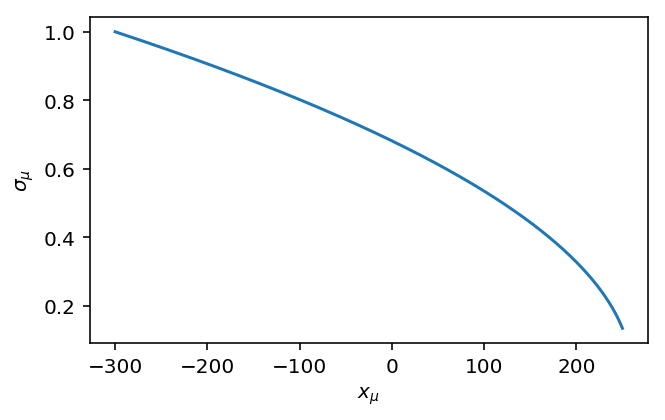
\includegraphics[width=0.4\linewidth]{pics/sigma.png}}
%\caption{$\sigma_{\mu}$}
%\label{fig:1}
%\end{figure}

Now we can introduce the complete loss function, that depends on the
physical performance of the shield, its weight and the length, the
later  implicitly via the weight.
\[
L(\Sigma, W) = (1 + \Sigma) (1 + \exp^{\frac{W - W_{0}}{W_{0}}}),
\]
where $\Sigma  = \sum_{\mu} \sigma_{\mu}$, $W$ is a weight of
configuration and $W_{0}$ is a weight of a baseline
configuration~\cite{Akmete:2017bpl} ahown in Fig.\ref{fig:baseline}. The weight of the baseline is about 1900 tons and $\Sigma$ is approximately equal to 32. As can be seen, weight is penalized exponentially because we are not interested in the heavy regions, as we will not be able to construct such configurations due to budget constraints.


\begin{figure}[H]
\center{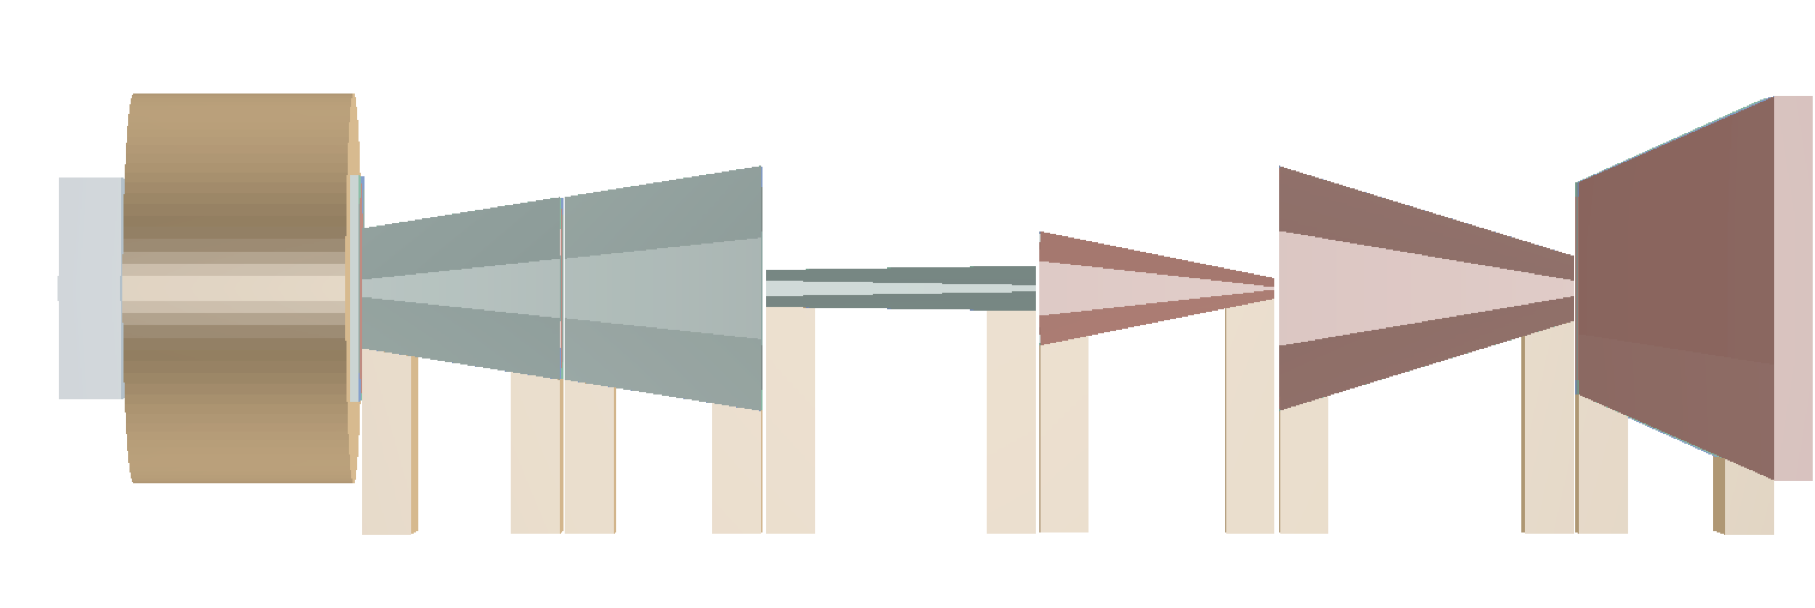
\includegraphics[width=0.4\linewidth]{pics/baseline.png}}
\caption{\label{fig:baseline}Baseline configuration}
\end{figure}

The following problems is addressed during the optimization:
\begin{enumerate}
\item Optimization is performed in 42-dimensional space
\item Computation of the $\Sigma$ is time consuming.
\item Computation of the $\Sigma$ is noisy due to limited statistics
  in Monte - Carlo simulations.
\end{enumerate}

We choose only 500k muons with the biggest momentum and discard
all the low-momentum muons. It helps us to decrease the time of
computations by factor of  8 times in average. We also introduce noise
as a prior knowledge into Gaussian Process: in this setup GP tries to
estimate the noise of the computation and incorporate it into final
variance. The points are computed in batches of 100 points to optimise
the usage of the available computing resources. The process of
optimization is illustrated in Fig.~\ref{fig:evolution}

\begin{figure}[H]
\center{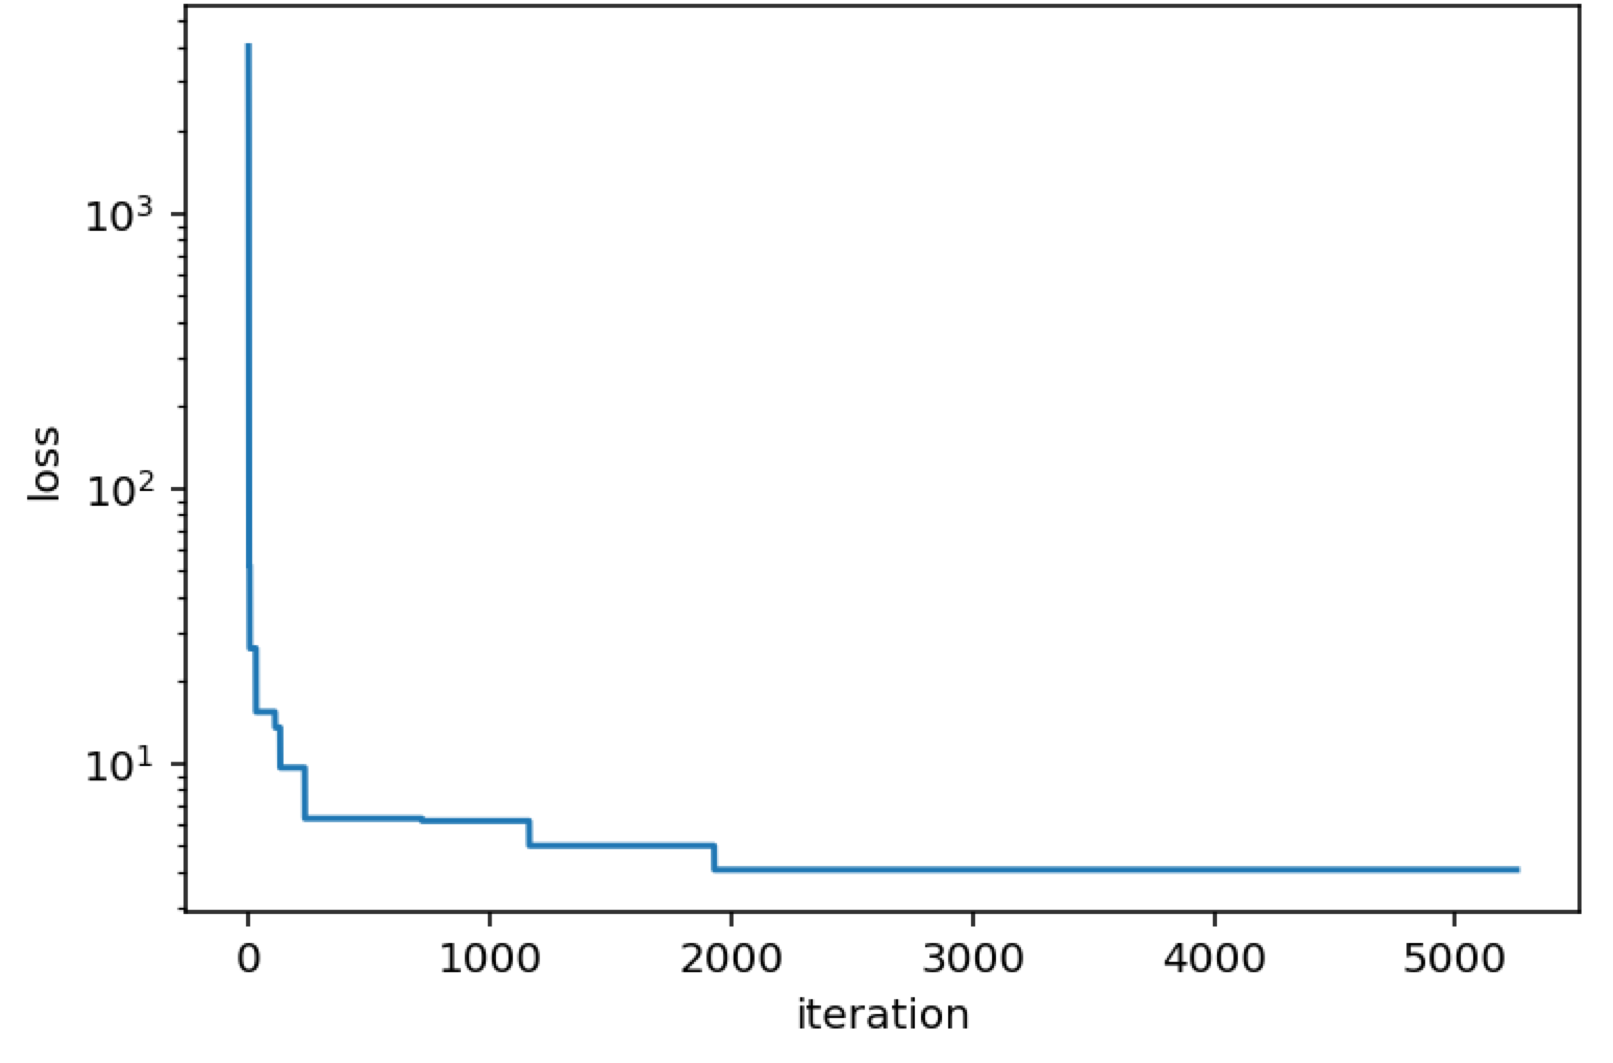
\includegraphics[width=0.4\linewidth]{pics/opt}}
\caption{\label{fig:evolution}Evolution of the best known point}
\end{figure}


The optimization procedure is stopped after 5000 iterations. 
The obtained configuration is found to be lighter by 25 \% than the baseline while having the same rejection capability. 

\begin{figure}[H]
\centering
\begin{minipage}[c]{0.45\textwidth}
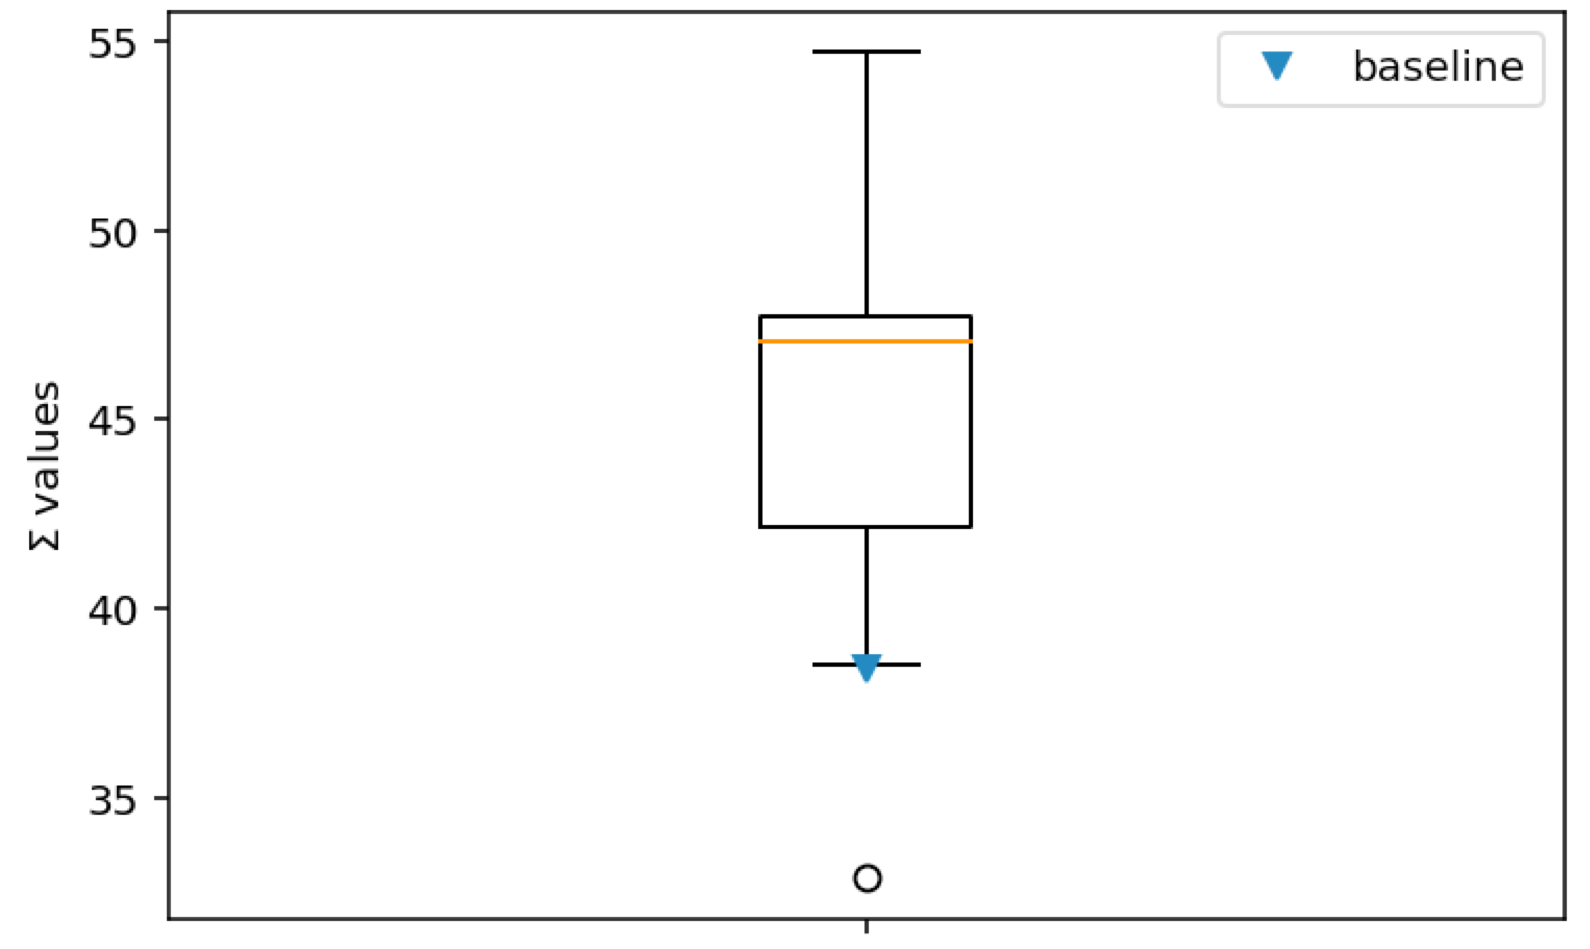
\includegraphics[width=0.9\textwidth]{pics/solution}
 \caption{\label{fig:sub1} Behaviour of the discovered configuration}
 \end{minipage}
\begin{minipage}[c]{0.45\textwidth}
  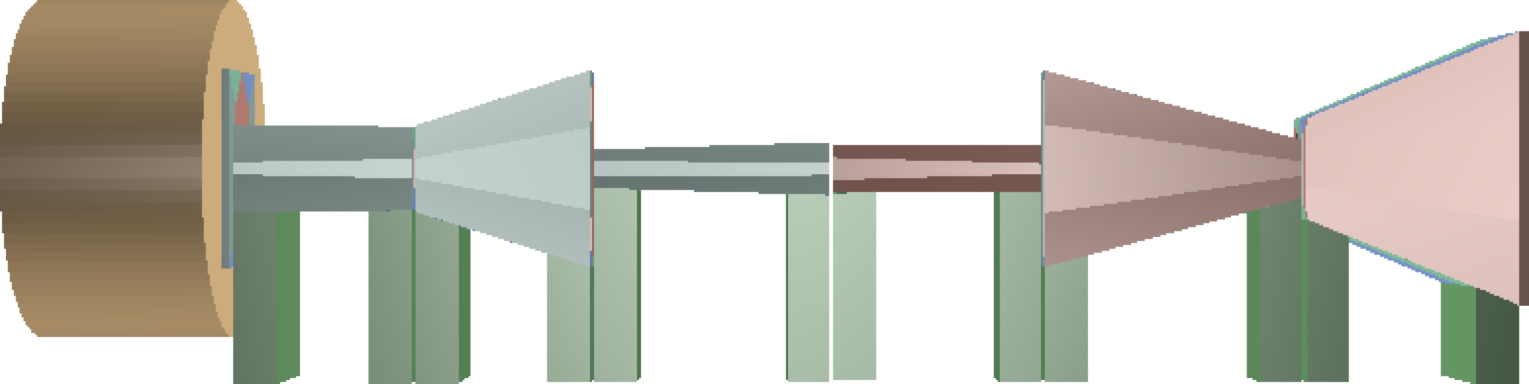
\includegraphics[width=0.9\textwidth]{pics/sol_2.png}
  \caption{\label{fig:sub2} Discovered configuration}
\end{minipage}  
\end{figure}

Fig.~\ref{fig:sub1} indicates the distribution of the $\Sigma$ for the
discovered configuration after multiple simulations with different
random seeds. We can see that the mean of the distribution is bigger
than $\Sigma$ for the baseline, but values are still low.  Fig.~\ref{fig:sub2} illustrates the new found configuration.

\section{Conclusion}

Bayesian optimization is a powerful tool which can be applied for the
optimization of non-differentiable functions. We have demonstrated
that this method can be successfully applied even to 
complicated optimization problems in physics. 
However in spite of GP can guarantee global optionality under ideal
conditions,  these are not satisfied for this particular problem.

\ack

\section*{References}

\begin{thebibliography}{9}
\bibitem{Ellis:2009tp} Ellis J {\it et. al} 2009 {\it Phys. Lett.} B {\bf679} 369-375
\bibitem{Asaka:2005pn} Asaka  {\it et. al} 2005 {\it Phys. Lett.} B {\bf 620} 17-26
\bibitem{Asaka:2005an} Asaka {\it et. al} 2005 {\it Phys. Lett.} B {\bf 631} 151-156
\bibitem{Bergsma:1985is} Bergsma F {\it et. al} 1986 {\it Phys. Lett.} B {\bf 166} 437-478
\bibitem{Bernardi:1985ny} Bernardi G {\it et. al} 1986 {\it Phys. Lett.} B {\bf 166} 479-483
\bibitem{Vaitaitis:1999wq} Vaitaitis A {\it et. al} 1999 {\it Phys. Rev. Lett.} {\bf 83} 4943-4946
\bibitem{CooperSarkar:1985nh} Cooper-Sarkar {\it et. al} 1985 {\it Phys. Lett.} B {\bf 160} 207-211
\bibitem{Bonivento:2013jag} Bonivento W {\it et. al} 2013 Proposal to Search for Heavy Neutral Leptons at the SPS {\it Preprint 1310.1762}
\bibitem{Burnaev2015} Burnaev E and Panov M {\it et. al} 2015 {\it Proc. SLDS 2015} (Egham) 116-125
\bibitem{Betro1991} Betr{\`o} B 1991 {\it J. of Glob. Opt.} {\bf 1} 1-14
\bibitem{rasmussen2006gaussian} Rasmussen C E and Williams C K I 2006 {\it Gaussian Processes for Machine Learning} (University Press Group Limited)
\bibitem{Mockus1994} Mockus J 1994 {\it J. of Glob. Opt.} {\bf 4} 347-365
\bibitem{Mockus1978} Mockus J, Tiesis V and Zilinskas A 1978 {\it Towards Global Optimization} {\bf 2} (Elsevier Science Ltd.) 117-129
\bibitem{vazquez2010convergence} Vazquez E and Bect J 2010 {\it J. of Stat. Plan. and Inf.} {\bf 140} 3088-3095
\bibitem{Akmete:2017bpl} Akmete A {\it et al.} 2017 {\it JINST} {\bf 12}

\bibitem{Pythia8}
Sj\"{o}strand T, Mrenna S, and Skands P  2008
\emph{Comput.Phys.Commun.} \textbf{178} 852-867

\bibitem{Genie}
Andreopoulos C, Bell A, Bhattacharya D, Cavanna F, Dobson J, {\it et al} 2010 \emph{Nucl.Instrum.Meth.} \textbf{A614} 87-104
\bibitem{Pythia6}
Sj\"{o}strand T, Mrenna S, and Skands P 2006 \emph{JHEP} \textbf{05} 026
\bibitem{Cascade}
Dijkstra H and Ruf T 2015 {\it SHiP-NOTE-2015-009}

\bibitem{Geant4}
Agostinelli S {\it et al.} 2003 \emph{Nucl.Instrum.Meth.} \textbf{A506} 250-303

\bibitem{FAIRROOT}
Al-Turany M Bertini D Karabowicz R Kresan D Malzacher P {\it et al.} 2012 \emph{J.Phys.Conf.Ser.} \textbf{396} 

\bibitem{Burnaev2016} Burnaev E Panov M and Zaytsev A 2016 {\it Journal of Communications Technology and Electronics} {\bf 61} 6 661-671.
\end{thebibliography}


\appendix

\end{document}